%!TEX root = main.tex
\section{Participants and Datasets\label{sec:participantdatasets}}
At the start of our design study, we observed participants as they conducted cognitive walkthroughs demonstrating their existing data analysis workflows. Next, we describe our study participants and their preferred analysis workflows.%use cases to highlight behaviors that participants have adopted for conducting certain analysis tasks.
\begin{table}[h!]
  \centering
  \vspace{-10pt}
  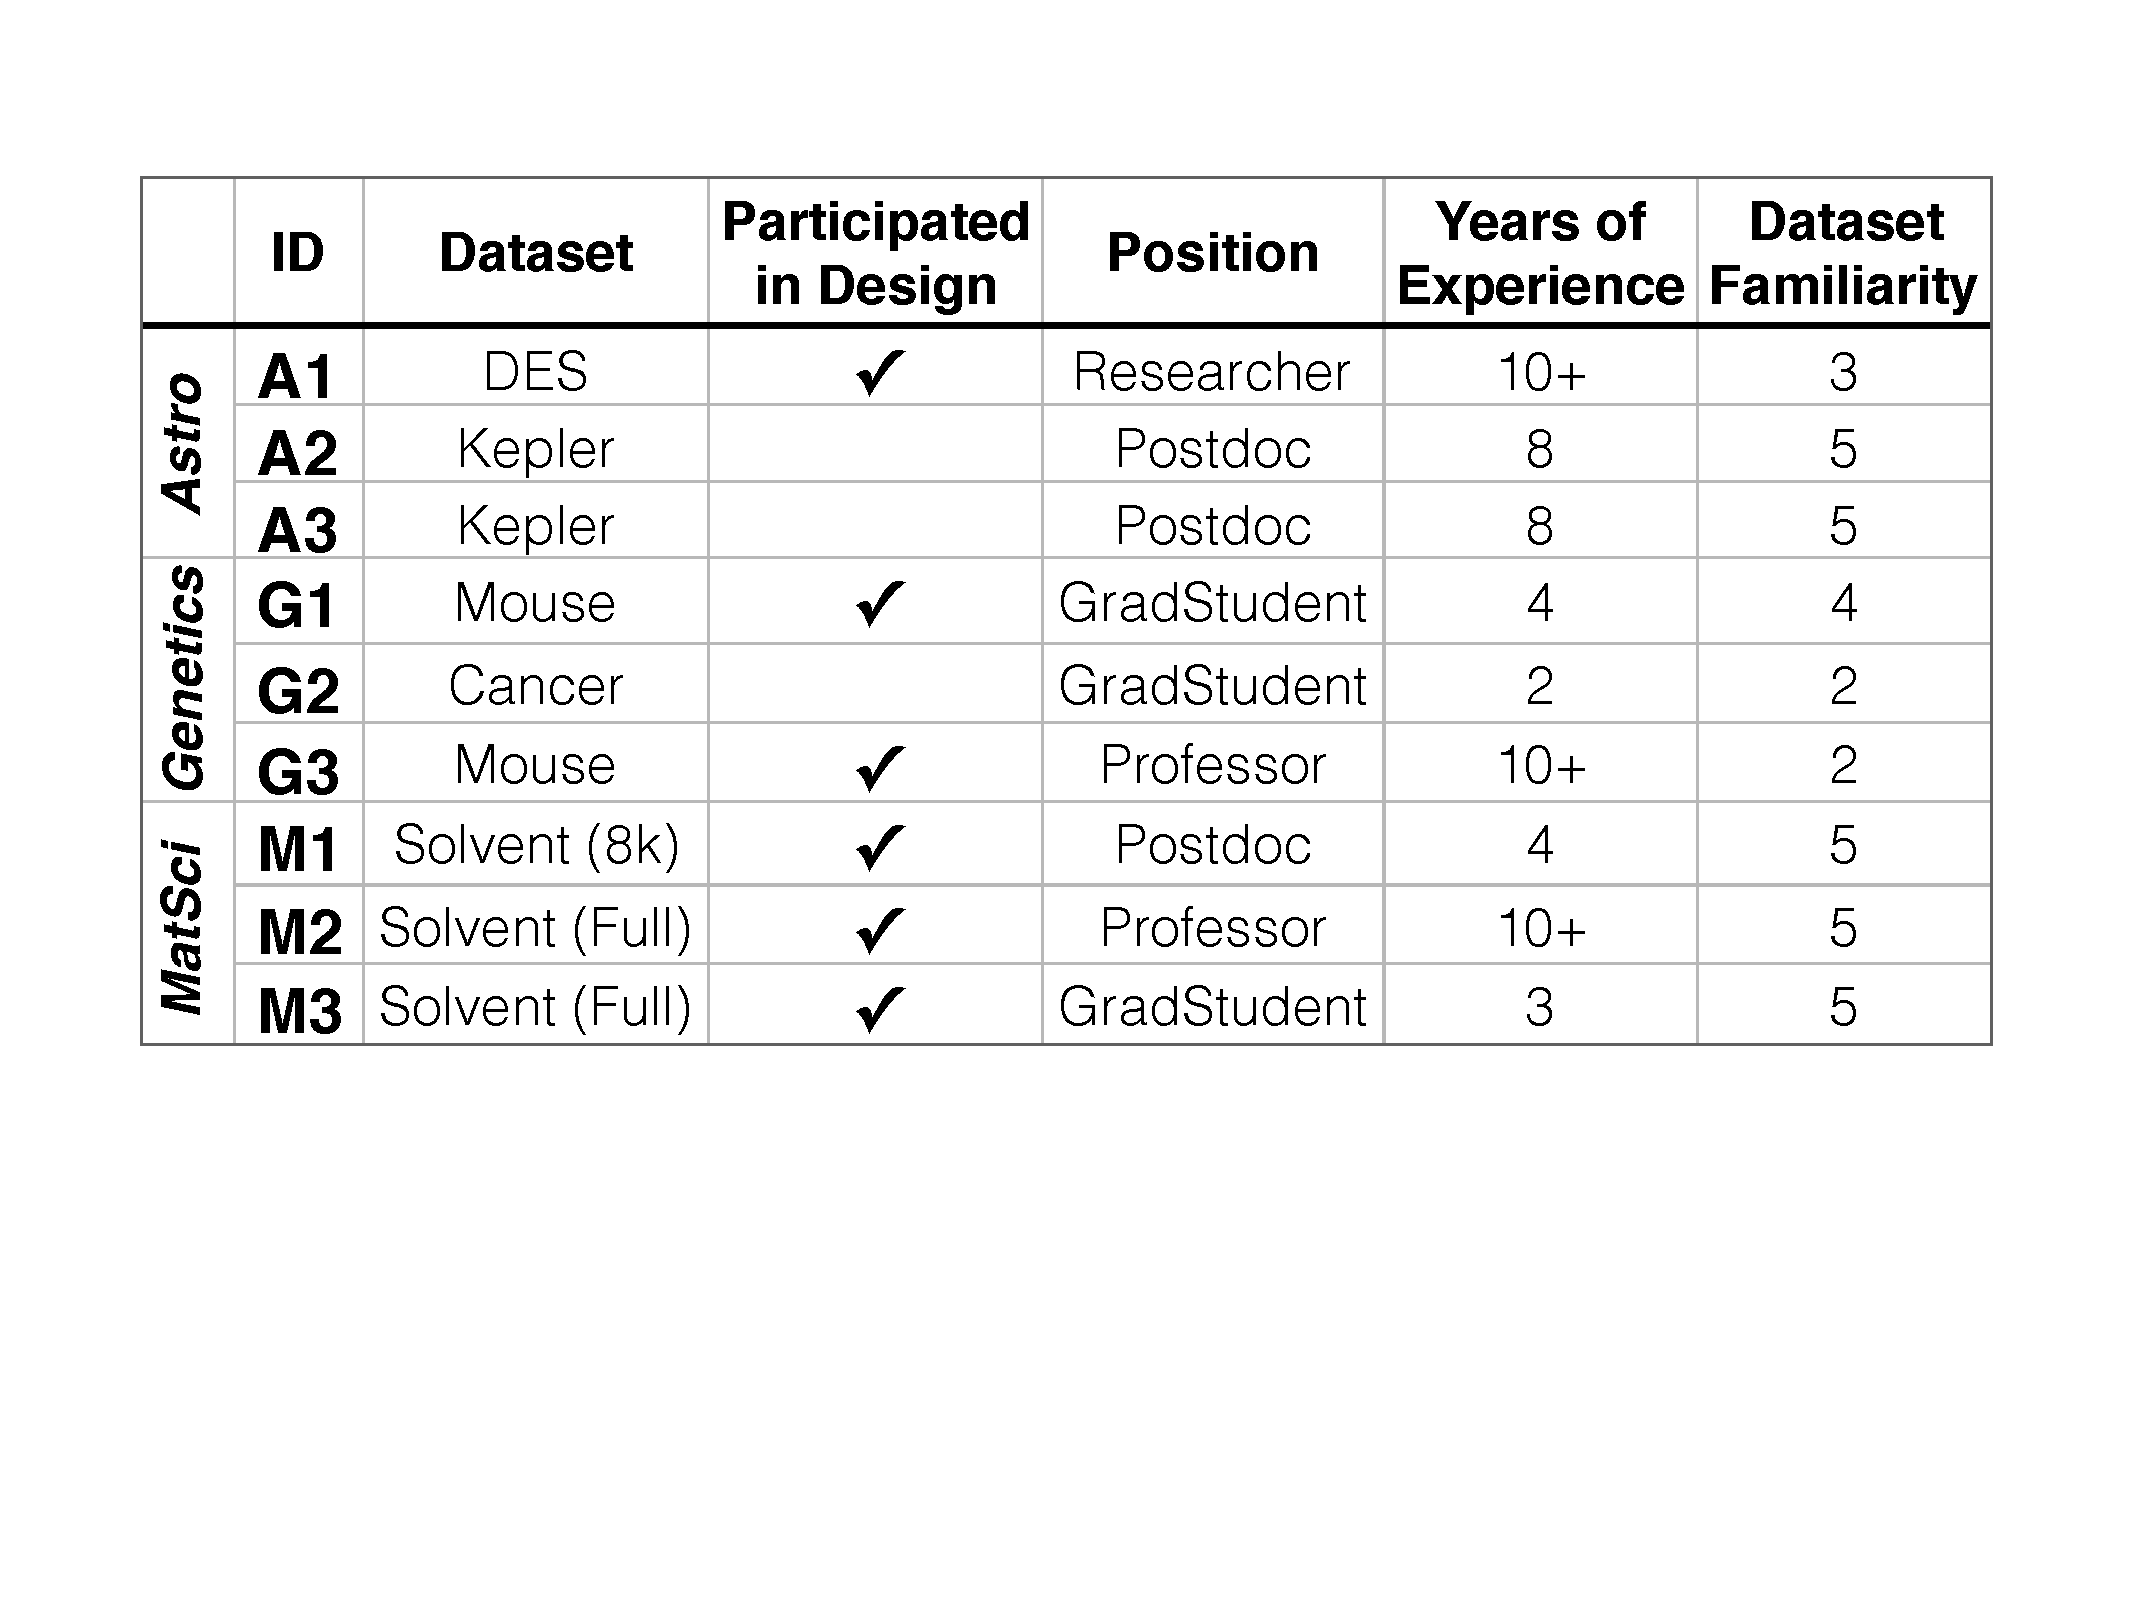
\includegraphics[width=\linewidth]{figures/participant_info.pdf}
  \caption{Participant information. The Likert scale used for dataset familiarity ranges from 1 (not familiar) to 5 (extremely familiar).}
  \label{participants}
  \vspace{-15pt}
\end{table}
\par\noindent\stitle{Astronomy:} The Dark Energy Survey is a multi-institution project that surveys 300 million galaxies over 525 nights to study dark energy~\cite{Drlica-Wagner2017}. The telescope used to survey these galaxies also focuses on smaller patches of the sky on a weekly interval to discover astronomical transients (objects whose brightness changes dramatically as a function of time), such as supernovae or quasars. Their dataset consists of a large collection of brightness observations over time, one associated with each astronomical object, called a {\em light curve}, and plotted as a time series. For over five months, we worked closely with A1, an astronomer on the project's data management team working at a supercomputing facility. Their scientific goal is to identify potential astronomical transients in order to study their properties. \techreport{These insights can help further constrain physical models regarding the formation of these objects.}
\par To identify transients, astronomers programmatically generate visualizations of candidate objects with \texttt{matplotlib} and visually examine each light curve. While an experienced astronomer who has examined many transient light curves can often distinguish an interesting transient object from noise by sight, manual searching for transients is time-consuming and error prone, since the large majority of the objects are false positives. A1 was interested in VQSs as he recognized how specific pattern queries could help astronomers directly search for these rare transients.
\techreport{\par If an object of interest or region is identified through the visual analysis, then the astronomer may be interested in inspecting the image of the region for cross-checking that the significant change in brightness of the object is not due to an imaging artifact. This could be done using a custom built web-interface that facilitates the access of cutout images for a queried region of the sky.}
\begin{figure*}[ht!]
  \centering
  \vspace{-5pt}
  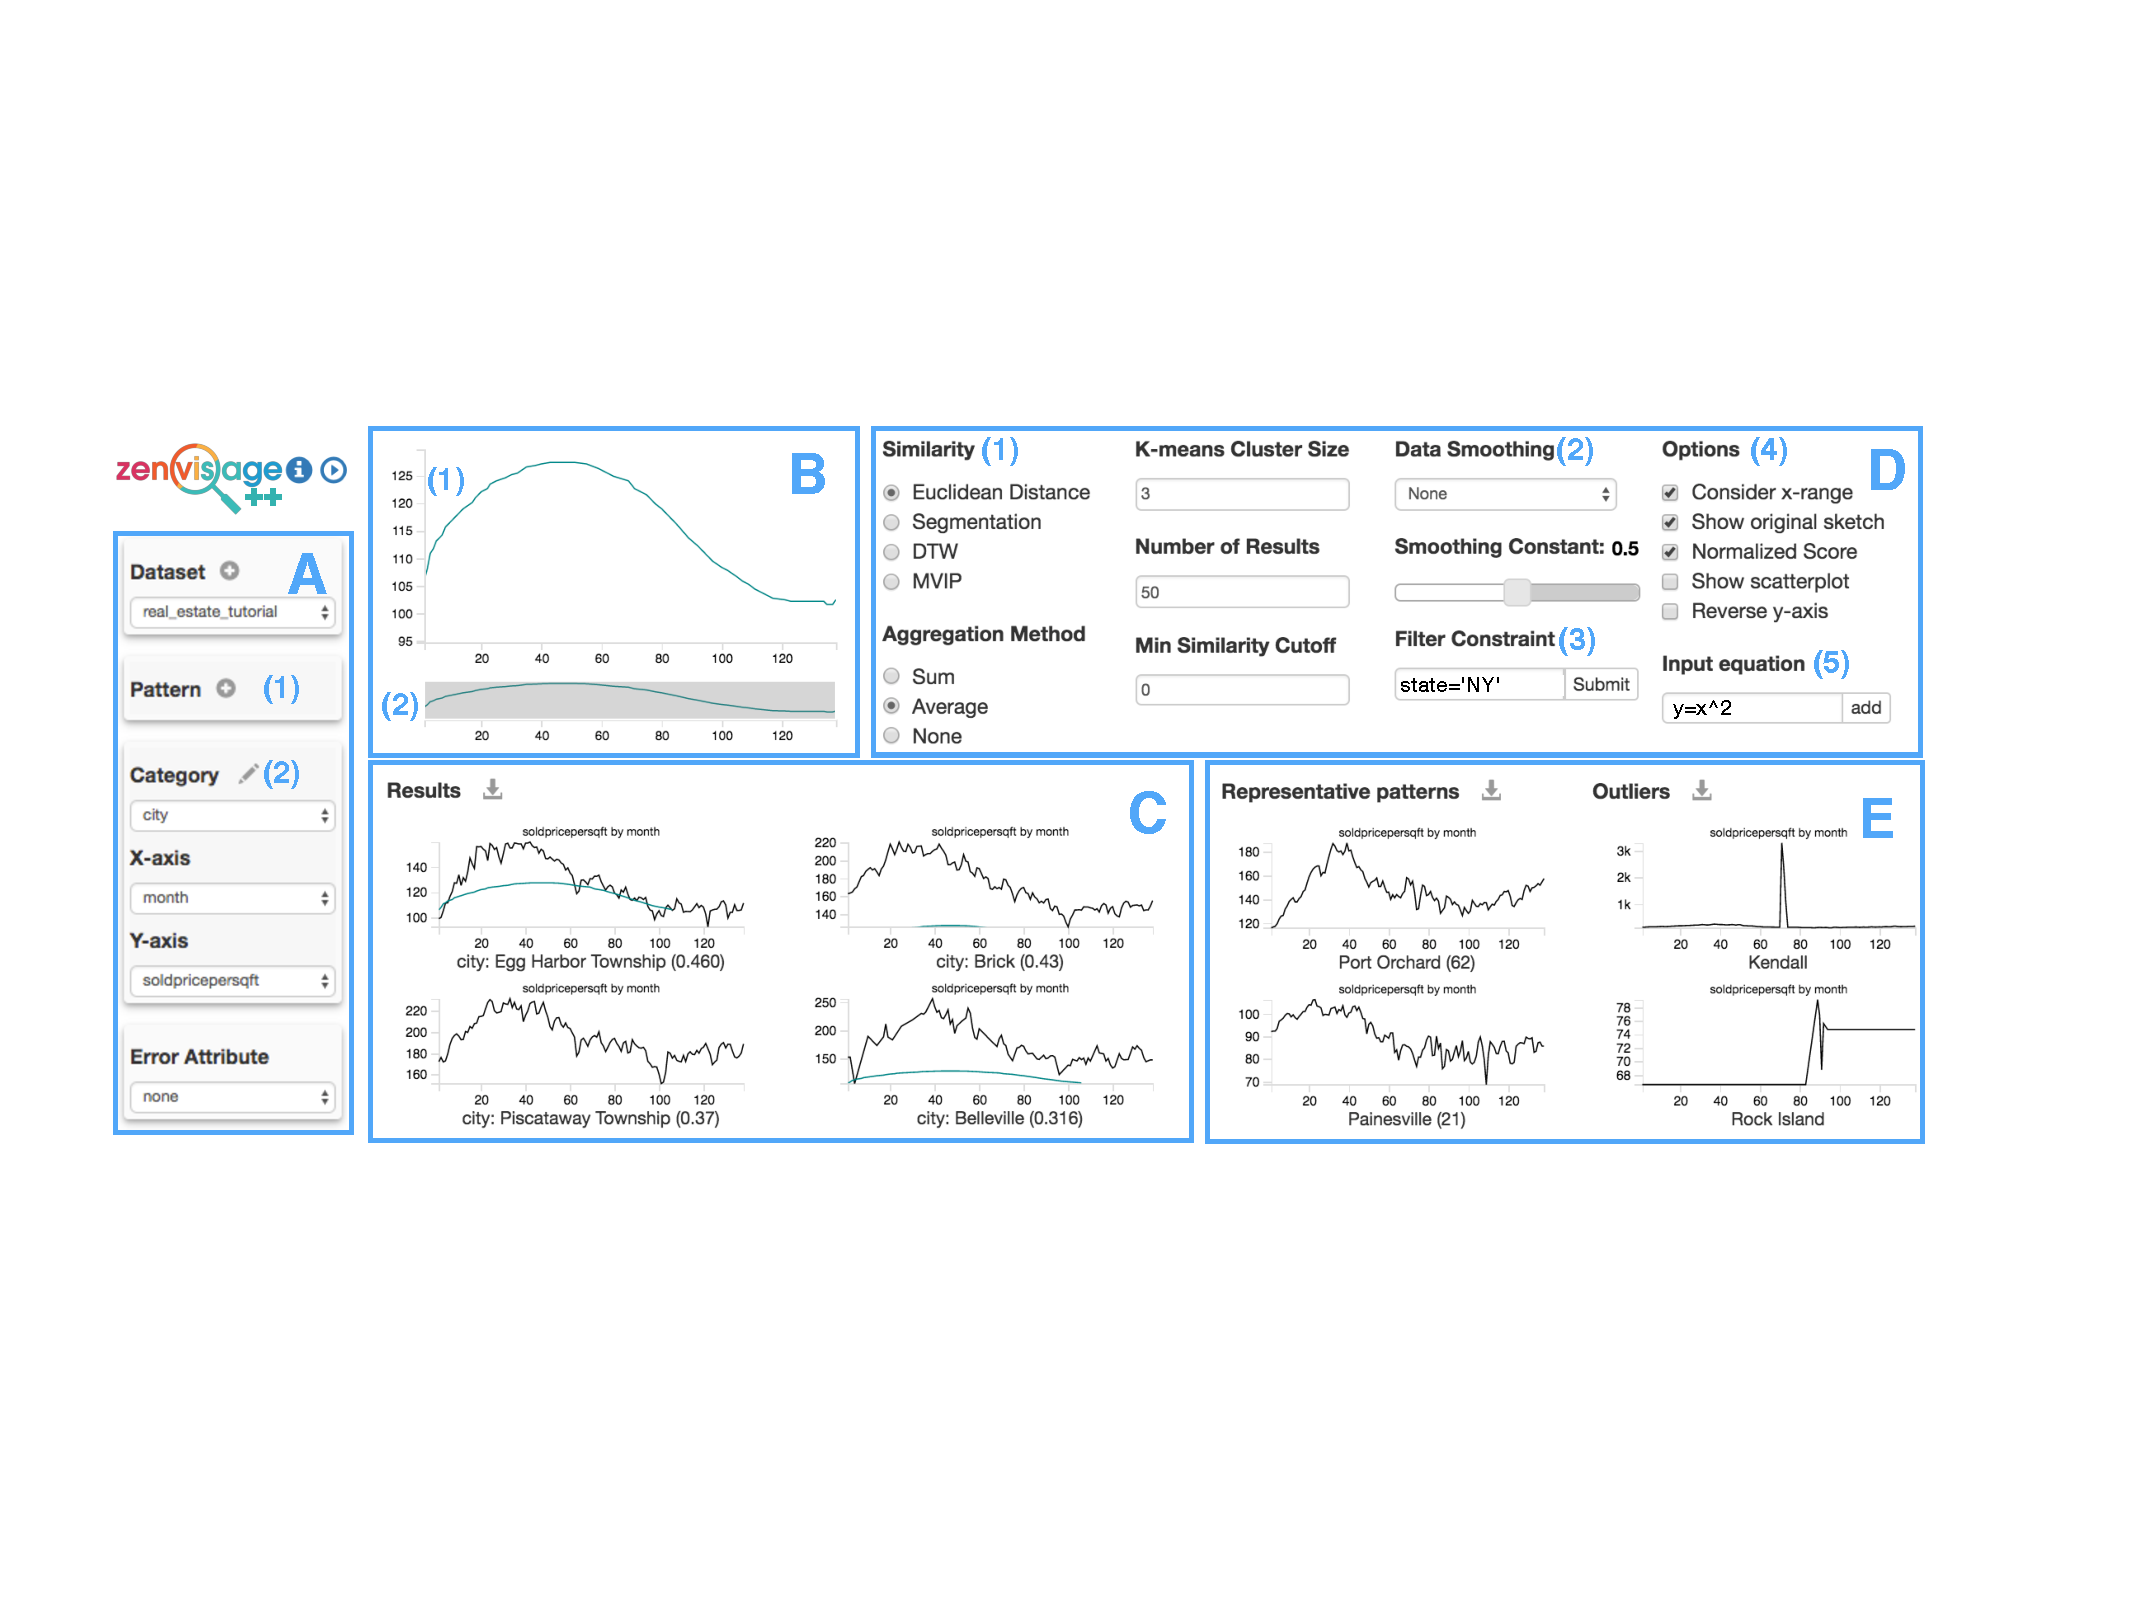
\includegraphics[width=0.95\linewidth]{figures/zvpp_system.pdf} %5.5
  \vspace{-5pt}\caption{The \zvpp system, including: the ability to query via (a) a sketch,(b) input equations, (i) uploaded patterns, or (j) drag and drop; (c) data smoothing; query specification mechanisms including (d) x-range selection and filtering, (e) x-range invariance, (f) similarity metric selection, (g) filtering, and (h) dynamic class creation; recommendation of (k) representative and (l) outlier trends.} %Prior to the participatory design, \zv only included a single sketch input with no additional options.}
  \label{zvOverview}
  \vspace{-5pt}
\end{figure*}
\par\noindent\stitle{Genetics:} Gene expression is a common measurement in genetics obtained via microarray experiments~\cite{Peng2016}. \techreport{In these experiments, a grid containing thousands of DNA fragments are exposed to stimuli and measurements for the level at which a gene is expressed are recorded as a function of time.} We worked with a graduate student (G1) and professor (G3) at a research university who were using gene expression data to understand how genes are related to phenotypes expressed during early development\techreport{\cite{Peng2016,Gloss2017}}. Their data consisted of a collection of gene expression profiles over time for mouse stem cells, aggregated over multiple experiments.\techreport{, downloaded from an online database\footnote{\url{ncbi.nlm.nih.gov/geo/}}.} %They were interested in using \zv to cluster gene expression data before conducting analysis with a downstream machine learning workflow.
\par Their typical workflow is as follows: G1 first loads the preprocessed gene expression data into a custom desktop application for visualizing and clustering it\techreport{\footnote{\url{www.cs.cmu.edu/~jernst/stem/}}}. After setting several system parameters and executing the clustering algorithm, the overlaid time series for each cluster is displayed on the interface. G1 visually inspects that the patterns in each cluster looks ``clean'' and checks that the number of outlier genes (i.e., those that do not fall into any of the clusters) is low.  If the number of outliers is high or the clustered visualizations look ``unclean'', she reruns the analysis by increasing the number of clusters. Once the visualized clusters look ``good enough'', G1 exports the clusters to her downstream regression tasks.
\par Prior to the study, G1 and G3 spent over a month attempting to determine the best number of clusters based on a series of static visualizations and statistics computed after clustering. While regenerating their results took no more than 15 minutes every time they made a change, the multi-step, segmented workflow meant that all changes had to be done offline.\techreport{, so that valuable meeting time was not wasted trying to regenerate results.} The team were interested in VQSs as they saw how interactively querying time series with clustering results could dramatically speed up their collaborative analysis process.
%that can improve battery performance and stability
\par\noindent\stitle{Material Science:} We collaborated with material scientists at a research university who are working to identify solvents for energy efficient and safe batteries. These scientists work on a large simulation dataset containing chemical properties for more than 280,000 solvents~\cite{Khetan2018}. Each row of their dataset represents a unique solvent with 25 different chemical attributes. We worked closely with a a postdoctoral researcher (M1), professor (M2), and graduate student (M3) for over a year to design a sensible way of exploring their data. They wanted to use VQSs to identify solvents that not only have similar properties to known solvents but are also more favorable (e.g., cheaper or safer to manufacture). To search for these desired solvents, they need to understand how changes in certain chemical attributes affect other properties under specific conditions.
\par M1 typically starts his data exploration process by iteratively applying filters to a list of potential battery solvents using SQL queries. When the remaining list of the solvents is sufficiently small, he examines each solvent in more detail to factor in the cost and availability to determine experimental feasibility. The scientists were interested in VQSs as it was impossible for them to uncover hidden relationships between different attributes across large number of solvents manually.%(such as how changing one attribute affects another attribute)
